\section{Pattern Analysis}

\begin{frame}{Pattern Analysis with EOF}
  \begin{columns}
    \begin{column}{.5\textwidth}
      \begin{itemize}
        \item For those familiar: it is related to PCA
        \item very widely used in geospatial sciences (see review paper from \citeauthor{hannachi_empirical_2007} \cite{hannachi_empirical_2007})
        \item can be used for dimensionality reduction, filtering, variability pattern recognition \dots
        \item already been used for IVT fields \cite{ayantobo_integrated_2022, salstein_modes_1983, jiang_water_2009}
%        \item also some interesting modifications: REOFs
      \end{itemize} 
      
    \end{column}
    \begin{column}{.5\textwidth}
    \begin{figure}[t]
      \centering
      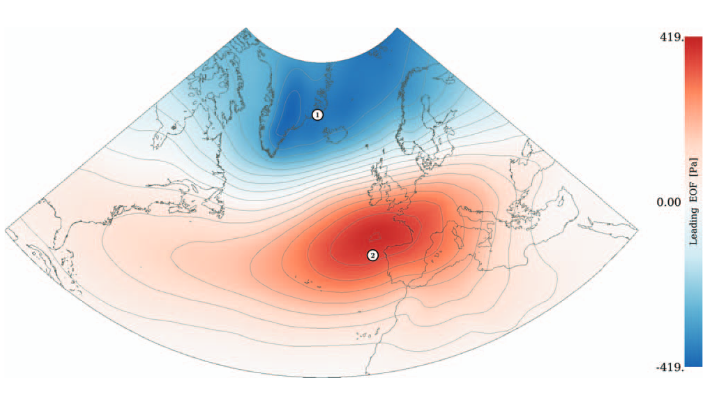
\includegraphics[width=.7\columnwidth]{imglib/nao_eof_index.png}\\
      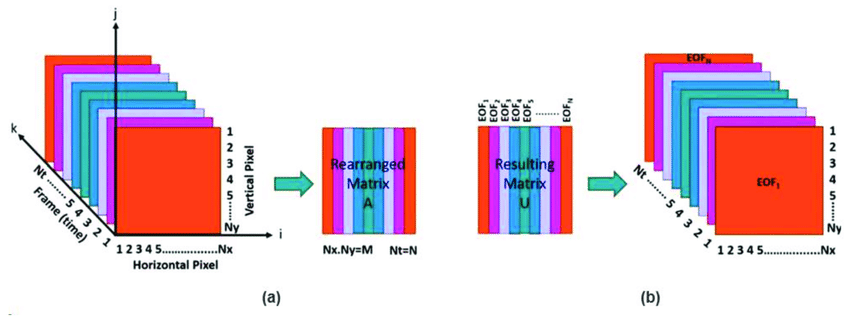
\includegraphics[width=.9 \columnwidth]{imglib/eof_matrix_decomp.png}
      {\tiny Source: \href{https://www.researchgate.net/publication/357212141_Latest_Advances_in_Common_Signal_Processing_of_Pulsed_Thermography_for_Enhanced_Detectability_A_Review/figures?lo=1}{researchgate}}
    \end{figure}

    \end{column}
    
  \end{columns}
\end{frame}

% \begin{frame}{My current plan}
%   
%   {\large
%   \begin{enumerate}
%     \item Filter the MPI-GE for my needs
%     \item Generate an IVT field from the MPI-GE
%     \item Implement a similar windowed EOF approach as in \cite{vietinghoff_visual_2021} to track changes in moisture transport patterns
%       \begin{itemize}
%         \item maybe apply concept of atmospheric rivers to the analysis
%         \item maybe also implement/use some other analyses from similar work 
%       \end{itemize}
%     \item Visualize the uncertain Scalar Fields over time
% %      \begin{itemize}
% %        \item some more open questions 
% %      \end{itemize}
%   \end{enumerate}
% }
% \end{frame}
